\pagenumbering{arabic}
\chapter{引~~言}\label{chap:introduction}


\section{课题背景}

\subsection{数字混沌系统动力学退化与抵抗}

混沌现象在自然界和数学模型中普遍存在,理解混沌现象中隐含的动力学行为很重要。作为非线性科学的一个令人难以置信的重要分支,混沌动力学是
自二十世纪70年代迅速发展起来的一门交叉科学,涉及生物学\upcite{Robert1976life}、化学\upcite{Zaikin1970chemistry}、物理学
\upcite{Otton1976physics,Hénon1976physics,Feigenbaum1978physics}、数学
\upcite{sharkovskii1964math,Yorke1975math,David1980math,AN1995math}和工程领域
\upcite{Lorenz1963engineering,Edward1963engineering},也是混沌理论和非线性科学领域的
基础课题\upcite{hao2013dynamics,hu2001chaos,SJ2003dynamics,XJ2011chaos}。由于混沌系统具有分形、初值敏感性和混沌吸引子等特性,
因此其动力学行为很难预测。混沌因此用于设计真随机数发生器、伪随机数发生器和安全保密通信算法。

当我们在数字计算机上模拟混沌时,相应的动力学系统会在时间和空间上被离散化\upcite{kocarev2006discrete,Blank1997Discreteness}。
对于数字化混沌系统而言,由于混沌系统都是在有限精度下实现的,数字设备的有限字长恶化了混沌系统的各项性能,降低了相关应用的效能
\upcite{Voss:computer:1989,umeno2013chaotic:TIT13}。尽管一些研究者指出如果数字计算机的字长足够大(例如,大于16位),
非线性混沌系统在计算机上有近似混沌行为,但在有限精度下数字混沌系统普遍存动力学特性退化\upcite{Persohn:AnalyzeLogistic:CSF12},
因为在有限精度数字域(或有限状态机)中舍入误差和截断误差(算法误差)会影响运算结果,使之与理论值存在偏差
\upcite{Oteo:error:PRE2007,Galias:rounding:CSM2013}。1988年,Yorke等人发现Ikeda映射的轨道周期的期望值随着舍入精度的变化
而变化\upcite{Yorke:Round:PRA88}。
为了理解连续混沌变为数字混沌的过程中混沌系统动力学的退化,2005年,S. LI等人提出一些度量分段线性混沌映射的动力学退化程度的客观指标
\upcite{Li:DPWLCM:IJBC2005}。混沌系统被广泛应用于安全保密通信算法,但数字混沌系统的动力学退化可能会大大降低混沌保密算法的安全性
\upcite{LiShujun:Rules:IJBC2006}。

\begin{figure}[!htb]
\centering
\begin{minipage}{\TwoImW}
\centering
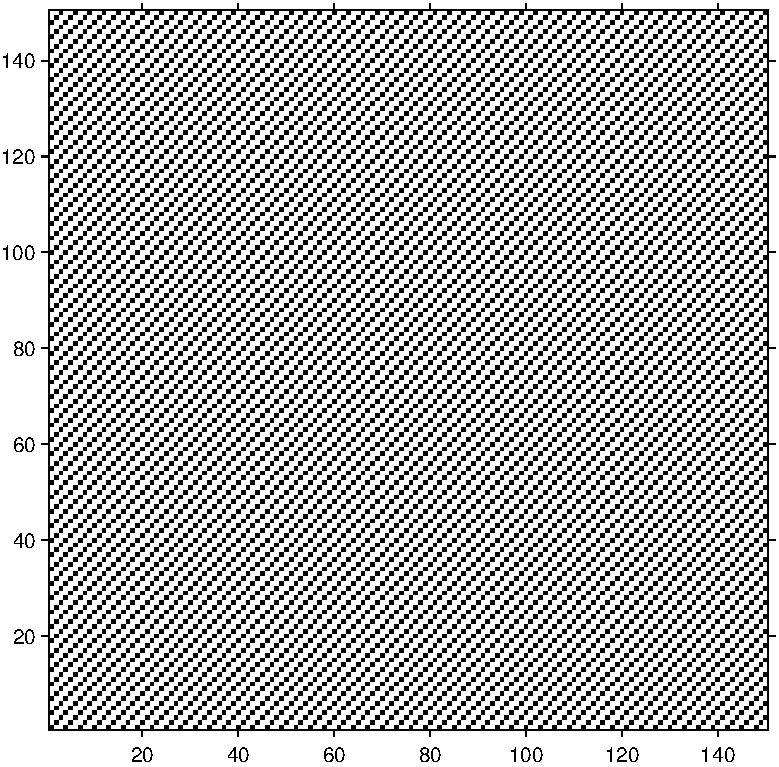
\includegraphics[width=\TwoImW]{Period_3}
a)
\end{minipage}\hspace{1mm}
\begin{minipage}{\TwoImW}
\centering
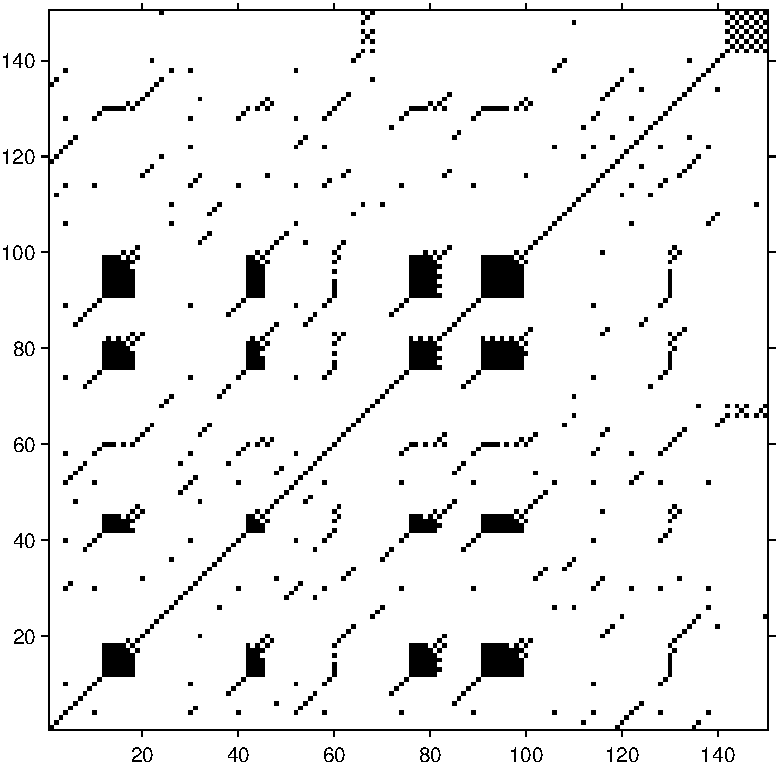
\includegraphics[width=\TwoImW]{Band_merging}
b)
\end{minipage}
\begin{minipage}{\TwoImW}
\centering
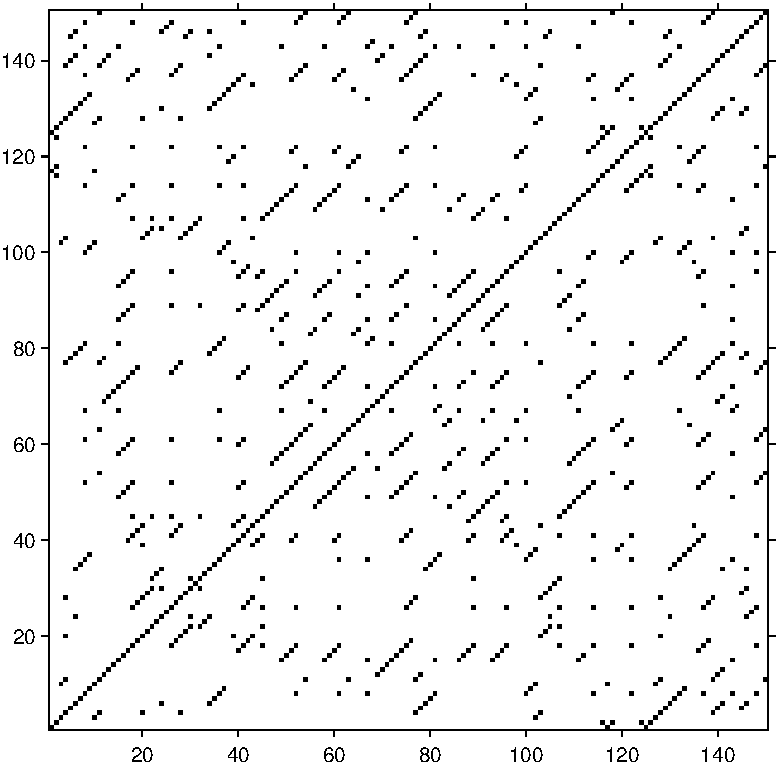
\includegraphics[width=\TwoImW]{Laminar}
c)
\end{minipage}\hspace{1mm}
\begin{minipage}{\TwoImW}
\centering
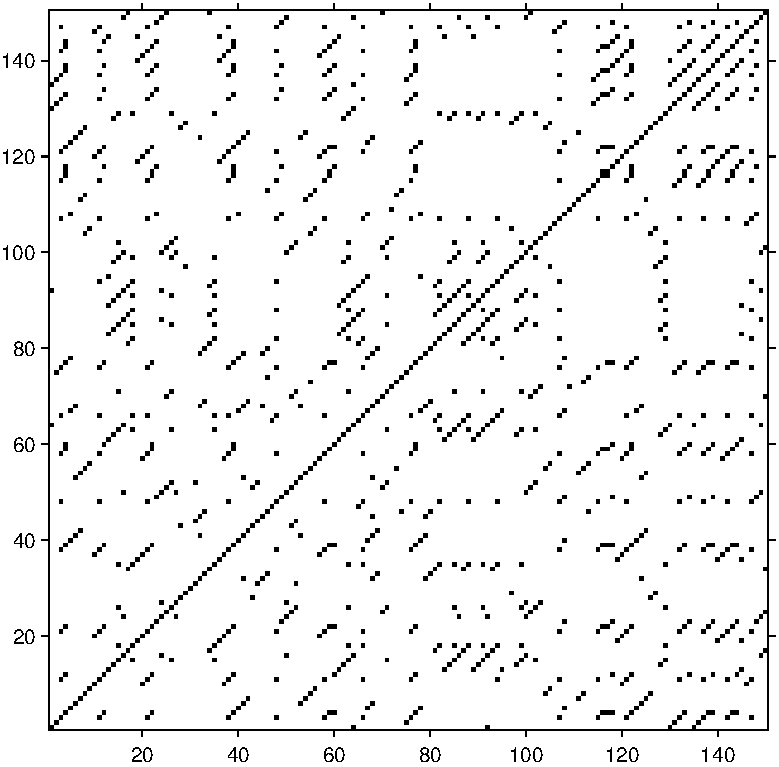
\includegraphics[width=\TwoImW]{Outer_crisis}
d)
\end{minipage}
\caption{Logistic映射不同动力学状态的递归图: a) $\mu=3.830$; b) $\mu=3.679$; c) $\mu=3.791$; d) $\mu=4$}
\label{fig:RP}
\end{figure}

为了抵抗数字混沌系统的动力学特性退化,各种各样的应对策略被提出:增大精度\upcite{lin1991chaos}、
扰动混沌状态\upcite{tao1998perturbance,heidari1994chaotic,Chen:random:CASII2010,LiCY:PRNS:VLSI2012}、
扰动控制参数\upcite{vcernak1996digital}、级联两个或多个混沌映射\upcite{Hua:model:CAS17}、
在多个混沌映射之间切换\upcite{nagaraj2008increasing,YCZhou:Switching:TCASI2014}和反馈控制
\upcite{addabbo2006feedback,HPhu:DCS:SMCS2015}。
上述方法通常被用于改善混沌伪随机数发生器的随机性能。许多研究者认为通过混沌迭代生成的伪随机数序列很大程度上保留了原始混沌映射
的复杂动力学特性\upcite{Phatak:LogisticRNG:PRE95}。事实上,早在1947年,John von Neumann已经提出将Logistic映射作为伪随机数发生器(PRNG)
\upcite{Neumann:logistic:BAMS47}。此后,大量基于混沌映射及其演化的伪随机数发生器(PRNG)被提出,例如
Logistic映射\upcite{heidari1994chaotic,Phatak:LogisticRNG:PRE95,Chen:random:CASII2010,LiCY:PRNS:VLSI2012,HPhu:DCS:SMCS2015}、
Tent映射\upcite{jessa2002periodtent,masuda2002cryptosystems,Addabbo:Tent:ITIM2006}、Sawtooth映射\upcite{jessa2006sawtooth}、
R{\'e}nyi混沌映射\upcite{addabbo2007class:TCASI}、Cat映射\upcite{Catchen2013period}等。当我们应用混沌伪随机数发生器生成伪随机数时
\upcite{kocarev2003pseudorandom,Addabbo:Tent:ITIM2006,HPhu:DCS:SMCS2015},面对如此多的可供选择的伪随机数生成器,一个很重要的问题是
如何简单有效地从本质结构上检测其随机性缺陷,并对其进行改进。

\begin{figure}[!htb]
\centering
\begin{minipage}{\TwoImW}
\centering
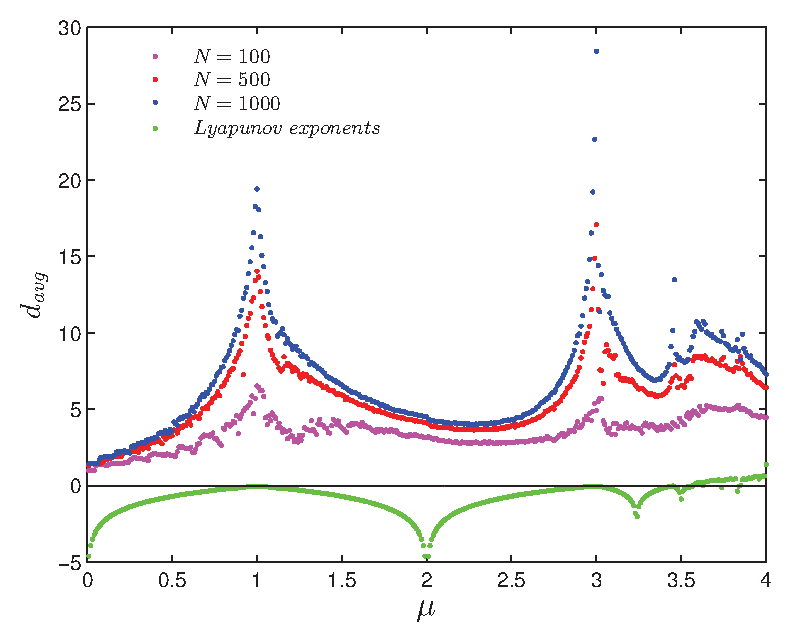
\includegraphics[width=\TwoImW]{davg}
a)
\end{minipage}\hspace{1mm}
\begin{minipage}{\TwoImW}
\centering
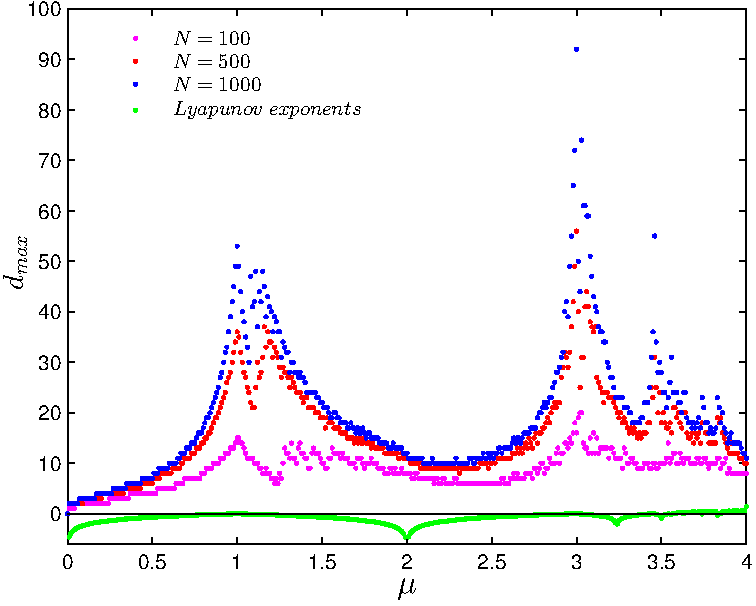
\includegraphics[width=\TwoImW]{dmax}
b)
\end{minipage}
\begin{minipage}{\TwoImW}
\centering
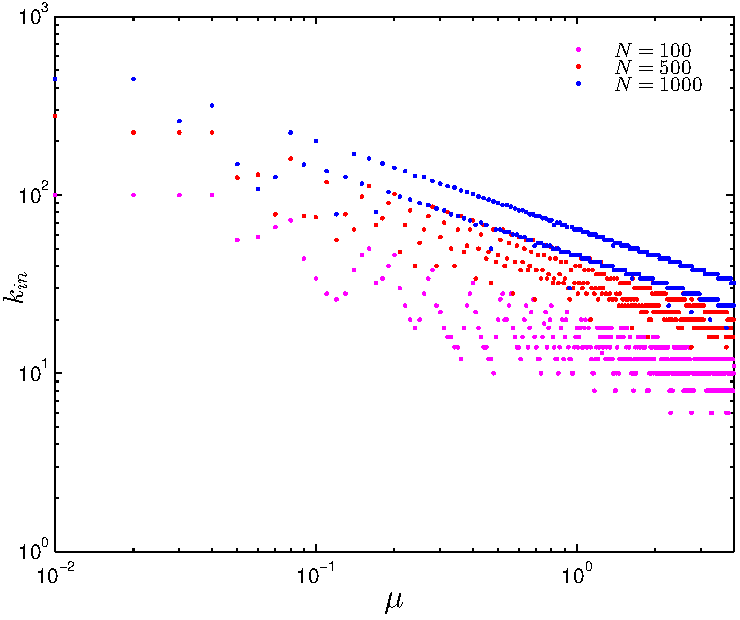
\includegraphics[width=\TwoImW]{kin}
c)
\end{minipage}\hspace{1mm}
\begin{minipage}{\TwoImW}
\centering
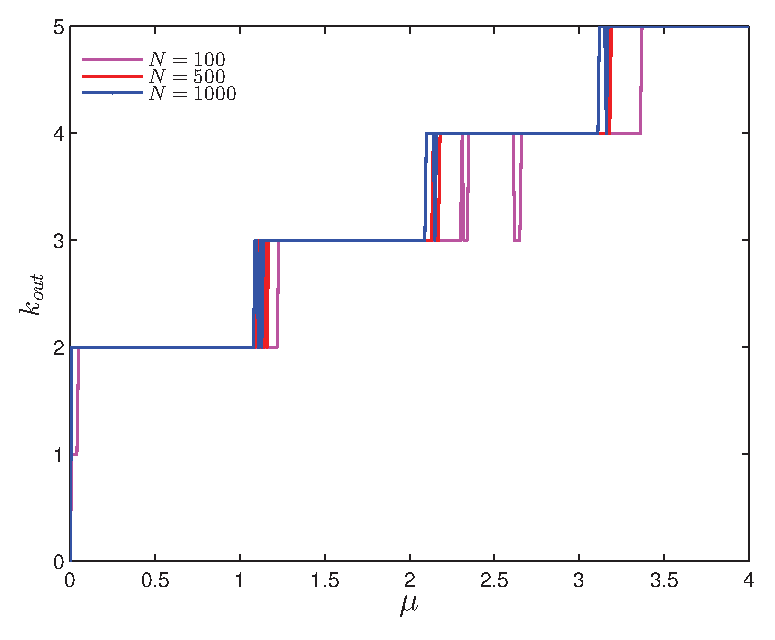
\includegraphics[width=\TwoImW]{kout}
d)
\end{minipage}
\caption{Logistic映射的子区间映射网络的不同参数指标随控制参数$\mu$的变化规律: a) 平均路径长度$d_{avg}$; b) 最大路径长度$d_{max}$;
c) 最大入度$k_{in}$; d) 最大出度$k_{out}$}
\label{fig:davg_dmax_kin_kout}
\end{figure}

\subsection{数字混沌系统动力学退化程度的刻画}

由于数字混沌系统动力学特性的退化对其在现实生活和工程领域中的应用有不可忽略的影响,对数字混沌动力学性质的研究开始受到人们的重视。
事实上,对数字混沌系统动力学性质分析的忽视是一些安全保密通信算法容易被破解的本质原因。
与混沌相关的早期研究发现,由于“鸽巢原理”和混沌系统可能状态的有限性,基于混沌迭代的伪随机状态序列经历一个暂态过程后将进入周期性循环
\upcite{sedgewick1982complexity,Philippe:Mapping:Crypto90}。
2007年,Oteo等人详细研究了Logistic映射在双精度计算中存在的舍入误差随控制参数的变化规律\upcite{Oteo:error:PRE2007}。
2011年,Takeru等人给出的实验结果表明,不同舍入方法对Logistic映射拟混沌轨道的暂态分枝长度和循环(\emph{cycle})长度有不同影响,
Logistic映射产生的状态序列的性质严重依赖于舍入方法\upcite{Takeru:Logistic:IEICE}。
2012年,Persohn等人使用高吞吐计算在单精度浮点域上穷举计算了Logistic映射拟混沌轨道的暂态分枝和循环\upcite{Persohn:AnalyzeLogistic:CSF12}。
2016年,Uehara等人揭示了Logistic映射的控制参数对其状态序列的暂态分枝长度和循环长度的影响\upcite{Uehara:logistic:ITA}。
Tsuchiya在2016年也给出有限域上控制参数为4的Logistic映射产生的状态序列周期的一些性质,并通过数值实验发现状态序列具有较长周期时控制参数
和初始值的条件以及周期的渐近性质\upcite{Kazuyoshi2016Logistic}。
2017年,X. Liao等人进一步推导出了有限域$\mathbb{Z}_{3^n}$上Logistic映射状态序列的最大周期\upcite{liao:period:SCIS17}。
此外,2012年、2013年,F. Chen使用Hensel上升法准确推导出了任意精度下二维离散Cat映射的周期分布,对离散Cat映射周期分布的充分认识有助于
Cat映射在水印和加密算法设计与分析中的应用\upcite{chen2012period,Catchen2013period}。
2016年,Yoshioka首先详细分析了2的整数幂余数环上切比雪夫多项式产生的状态序列的周期性质,分析表明,基于2的整数幂余数环上切比雪夫多项式的
公钥密码系统并不安全\upcite{Yoshioka2016Chebyshev}。最近,他又进一步推导出了奇素数的整数幂余数环上切比雪夫多项式的状态序列周期
\upcite{Yoshioka2018Chebyshev}。

\begin{figure}[!htb]
\centering
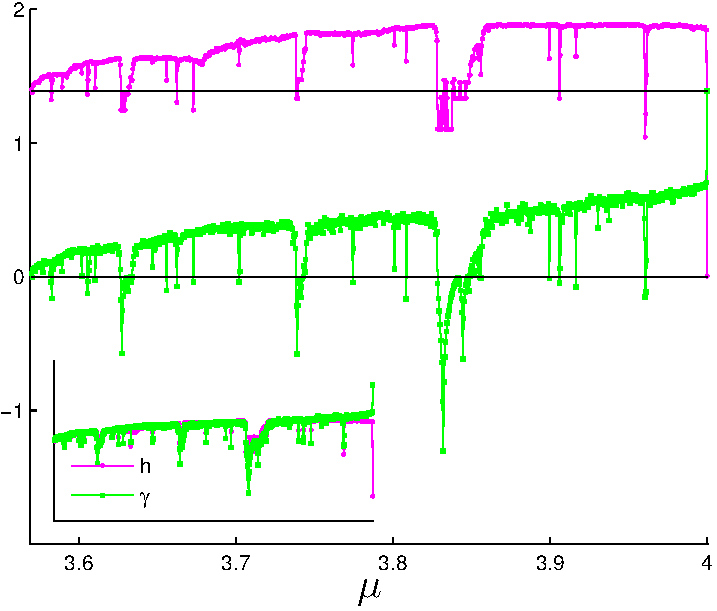
\includegraphics[width=1.25\BigOneImW]{Shannon_Lyapunov_Final}
\caption{Logistic映射网络熵$h$和Lyapunov指数$\gamma$随控制参数$\mu$的变化规律}
\label{fig:Shannon_Lyapunov}
\end{figure}

很多研究者侧重于状态网络中路径的分析,常常忽略数字域上给定混沌映射的所有可能状态之间的网络关系的存在\upcite{ozturk2014cycle}。
由于复杂网络可以用来研究传统理论数学模型不能准确描述的复杂非线性系统
\upcite{XJ2011chaos,Zhang:NetworkTimeSeries:PRL2006,Iba:LogisticNetwork:arxiv10,Borges:Mapping:EPJB07,Iba:NetworkChaos:ICCS2011},
它已经成为研究混沌系统动力学的有效工具。
1986年,Binder等人绘制了5比特定点运算域上Logistic映射的状态网络,从复杂网络的角度对其动力学特性进行了分析,并指出
混沌动力学特性的一些度量指标同样适用于状态映射网络(SMN),如李雅普诺夫指数和熵\upcite{Binder:Logistic:PRA86}。
1992年,Binder等人通过实验进一步研究了极限环数量和最大环周期随定点精度的变化规律\upcite{Binder:cycles:PHyD1992}。
2007年,Shreim等人通过复杂网络参数对基于元胞自动机的时间序列动力学进行了分类\upcite{Shreim:NetworkCA:2007},但C. Xu发现其中一些理论分析是错误的,
基于状态映射网络的两个参数指标不能区分由一维元胞自动机组成的离散动力系统的复杂动力学行为\upcite{XuC2017network}。
Kyriakopoulos和Thurner也通过子区间映射网络进一步探讨了复杂网络参数与混沌动力学特性度量指标之间的一致性(详见图~\ref{fig:davg_dmax_kin_kout})
\upcite{Thurner:Logistic:ICCS2007}。
2008年,X. Xu等人研究了混沌映射状态网络中指定4节点子图的相对频率,并根据指定4节点子图的相对频率对混沌映射进行了重新分类\upcite{xu:motif:PNAS08}。
2011年,Luque等人通过Feigenbaum图揭示了网络熵随控制参数的变化规律,发现其与李雅普诺夫指数随控制参数的变化规律相似
(详见图~\ref{fig:Shannon_Lyapunov})\upcite{Luque:FeigenbaumChaos:PLOS11}。
此外,为了进一步挖掘隐含在非线性时间序列中的重要信息,Donner等人在2011年提出了一种基于网络的非线性时间序列分析框架(详见图~\ref{fig:RP})
\upcite{Donner:GeometryDynamics:EPJB2011}。

尽管在数字混沌动力学领域有为数不多的研究者考虑过这个问题,我们认为关于数字混沌系统动力学性质的讨论是非常重要的。
更重要的是,在非线性科学领域,大多数人并不关心计算机如何执行浮点运算,而是将计算机作为黑匣子来实现混沌系统,
因此,在计算机上实现的数字混沌系统的本质结构仍未可知。此外,由于随机实验的局限性,很多研究者常常忽略可能以很低概率出现的某些重要细节。

\section{主要内容}

本文将以一维Logistic映射、Tent映射和二维离散Cat映射为主要分析对象,从状态映射网络的角度出发研究数字域上混沌系统的动力学性质,论文后续章节的内容安排如下:

第二章首先揭示了定点运算域上一维混沌系统状态映射网络的基本性质,对定点运算域上Logistic映射的SMN\ $F_e$与SMN\ $F_{e+1}$对应节点间的关系进行了具体分析;
其次,从理论上推导出了定点运算域上Logistic映射状态网络的节点入度分布和累积入度分布,发现Logistic映射状态网络具有无标度属性;然后,以Logistic映射为例
厘清了浮点运算域上系统量化误差对运算的影响,发现运算顺序和参与运算的数值范围会对运算结果产生影响,即改变运算顺序,运算结果可能不同;最后,利用有限域上混沌系统
的状态映射网络对混沌伪随机数发生器进行了分类,分析发现,混沌系统状态映射网络可对其随机性能进行粗检测。

第三章主要讨论了分段线性Tent映射的相关动力学性质,首先推导分析了定点运算域上其SMN\ $F_e$与SMN\ $F_{e+1}$对应节点间的准确关系;其次,揭示了定点运算域上
Tent映射状态网络的节点入度分布和累积入度分布,发现其节点入度仅有三种可能取值;然后,从理论上推导出了计算机内存中Tent映射迭代初值$x(0)$尾数位的无效位数$i$
的数学期望及$x(0)$的阶码$e$的数学期望,进而推导出了数字计算机上Tent映射迭代值趋于零所需迭代次数;最后,厘清了定点运算域上混沌系统状态映射网络与浮点运算域上
其对应状态映射网络之间的关系,即浮点运算域上混沌系统状态映射网络可由定点运算域上其对应状态映射网络生成。

第四章首先厘清了F. Chen等人于2013年提出的有限域上周期为$T$的不同Cat映射的数量$N_T$与二维离散Cat映射周期$T$之间的关系;其次,采用降维的方法对
定点运算域上二维离散Cat映射SMN\ $F_e$与SMN\ $F_{e+1}$之间的关系进行了深入分析;最后,通过随机实验揭示了二维离散Cat映射的环分布规律,发现其环分布呈
指数为1的幂律分布。

最后一章总结全文,对本文研究过程中遇到的一些问题进行了归纳整理。